% =============================================================================
%  北京市住房价格影响因素分析 —— 基于特征价格模型的多重回归实证研究
%  现代回归分析 课程论文
%  编译方式: xelatex -> xelatex (两次)
% =============================================================================

\documentclass[12pt,a4paper]{ctexart}

% ── 页面设置 ──
\usepackage{geometry}
\geometry{left=2.5cm, right=2.5cm, top=2.5cm, bottom=2.5cm}
\usepackage{setspace}
\onehalfspacing

% ── 字体 ──
\setCJKmainfont{SimSun}[ItalicFont={KaiTi},BoldFont={SimHei}]      % 正文宋体
\setCJKsansfont{SimHei}[BoldFont={SimHei}]                           % 无衬线黑体
\setCJKmonofont{FangSong}                                            % 等宽仿宋

% ── 数学 ──
\usepackage{amsmath,amssymb,bm}

% ── 图表 ──
\usepackage{graphicx}
\usepackage{caption}
\usepackage[table]{xcolor}
\usepackage{booktabs,array,tabularx}
\usepackage{longtable}
\usepackage{float}

% ── 超链接 ──
\usepackage[colorlinks=true,linkcolor=black,citecolor=black,urlcolor=black]{hyperref}

% ── 首行缩进 ──
\usepackage{indentfirst}
\setlength{\parindent}{2em}

% ── 标题格式 ──
\usepackage{titlesec}
\titleformat{\section}{\centering\sffamily\Large\bfseries}{\thesection}{1em}{}
\titleformat{\subsection}{\sffamily\large\bfseries}{\thesubsection}{1em}{}
\titleformat{\subsubsection}{\sffamily\normalsize\bfseries}{\thesubsubsection}{1em}{}

% ── 页眉页脚 ──
\pagestyle{plain}

% ── 图表路径 ──
\graphicspath{{../output/figures/}}

% =============================================================================
\begin{document}

% ──────────────────────────────
%  标题
% ──────────────────────────────
\begin{center}
{\sffamily\bfseries\zihao{-2} 北京市住房价格影响因素分析}\\[0.6cm]
{\sffamily\zihao{-3} ——基于特征价格模型的多重回归实证研究}\\[1.2cm]
{\zihao{4} 现代回归分析 课程论文}\\[0.3cm]
{\zihao{-4} 2026 年 4 月}
\end{center}

% ──────────────────────────────
%  摘要
% ──────────────────────────────
\section*{摘\quad 要}
\addcontentsline{toc}{section}{摘要}

住房价格的形成机制是城市经济学与房地产研究的核心议题。本研究基于链家平台
2011至2017年北京市二手房交易数据，在特征价格模型的理论框架下，综合运用
OLS回归、Ridge回归、LASSO回归、逐步变量选择及多项式扩展等多种方法，系统考察了
影响北京市住房价格的关键因素及其边际效应。研究得到以下主要发现。空间因素是解释
房价差异的主导变量，呈现显著的单中心城市空间衰减格局。交易年份对价格具有强预测
能力，但其影响呈现明显的非线性特征，若采用线性趋势设定将产生偏倚风险。房屋属性
方面，有无电梯、临近地铁、梯户比等变量对价格具有统计显著且经济含义清晰的边际贡献。
在模型比较层面，OLS与多项式组合模型取得了最优预测性能，但其系数因高阶项引发的严重
多重共线性而显著偏离经济直觉，模型的可解释性受到根本性损害。诊断检验表明数据存在
显著异方差和不同程度的多重共线性，经HC3稳健标准误修正后仅一个变量的显著性判断发生
改变，表明推断结果整体稳健。综合预测精度与经济可解释性，本文推荐以纳入区域和时间
双向固定效应的线性主效应模型作为结论支撑。

\noindent\textbf{关键词：}特征价格模型；住房价格；多重共线性；LASSO回归；稳健标准误；固定效应

\newpage

% ──────────────────────────────
%  一、引言
% ──────────────────────────────
\section{引言}

\subsection{研究背景}

住房兼具消费属性与投资属性，其价格形成机制一直是城市经济学、房地产金融学和应用统计学
共同关注的核心议题。北京市作为中国的政治、文化和国际交往中心，其房地产市场具有特殊
的典型意义。2011至2017年间，北京二手房市场经历了从温和上涨到加速攀升的转变：
安居客等平台数据显示，北京二手房均价从2011年的约2.5万元/m$^{2}$上升至2017年的约
6万元/m$^{2}$，年均涨幅超过15\%。这一轮房价上涨伴随着快速城镇化、宽松货币政策和
房地产市场调控政策（如2011年的「京十五条」限购政策、2013年的「国五条」、2016年的
「9·30新政」）的交替作用，呈现出典型的政策周期性特征。

在此背景下，准确识别住房价格的影响因素并量化其边际效应，不仅具有学术价值，也对
房地产估值、税收评估和住房政策制定具有重要的实践意义。

\subsection{文献综述}

住房价格研究的经典理论框架是特征价格模型，该模型由
Rosen（1974）在 Lancaster（1966）的消费者理论基础上系统发展而来。其核心思想是：
异质性商品的价格由其包含的一系列特征隐含的价格决定，因此可以通过回归方法估计各
特征的隐含价格。这一框架已被广泛应用于住房市场研究（Sirmans et al., 2005;
Bourassa et al., 2011）。

在实证方法层面，国内外学者不断拓展特征价格模型的分析工具。在变量选择方面，LASSO
回归（Tibshirani, 1996）通过L1惩罚实现自动变量选择，适用于高维特征场景；逐步回归
基于信息准则筛选变量，在传统经济计量中仍有广泛应用。在模型诊断方面，
Breusch-Pagan检验（Breusch \& Pagan, 1979）和White稳健标准误（White, 1980）已成为
异方差处理的标准工具；Cook距离（Cook, 1977）是识别强影响点的经典方法。

国内住房价格研究方面，郑思齐等（2005）较早采用特征价格模型分析北京住房市场；
龙奋杰和郑思齐（2007）系统梳理了特征价格模型在城市研究中的应用；张川川等（2016）
利用微观交易数据研究了限购政策对房价的影响。然而，已有研究较少在同一框架内系统
比较多种回归方法（正则化、变量选择、多项式扩展）的表现差异，也往往忽视了高缺失率
变量的处理偏倚和复杂模型的可解释性损失。本研究旨在弥补上述不足。

\subsection{研究框架与贡献}

本研究在特征价格模型的理论框架下，基于链家北京2011--2017年微观交易数据，构建了
从数据预处理、探索性分析、变量选择、模型诊断到多模型比较的完整回归分析流程。本研
究的主要贡献体现在以下三个方面。其一，系统比较了六种回归模型在预测精度与经济可解释
性之间的权衡，揭示了不同模型在两个维度上的优劣排序及其内在原因。其二，深入分析了
高缺失率变量（DOM缺失率50\%）的处理偏倚以及多项式模型中因多重共线性引发的系数
膨胀问题，为同类研究的方法选择提供了经验证据。其三，在模型评估中不仅关注
$R^{2}$和RMSE等预测指标，更强调核心变量的半弹性解释及其经济学
含义，力求在预测精度与经济可解释性之间寻求恰当的平衡。

% ──────────────────────────────
%  二、数据来源与预处理
% ──────────────────────────────
\section{数据来源与预处理}

\subsection{数据来源与说明}

本研究使用链家北京二手房交易数据，时间跨度为2011年至2017年。原始数据包含约32万条
交易记录和26个变量，涵盖房屋属性、交易属性、地理位置和社区特征四个维度的信息。
响应变量为每平方米价格，经对数变换后作为回归目标。

数据概况如下：原始样本量为318\,621条，价格均值为43\,562元/m$^{2}$，中位数为
38\,752元/m$^{2}$，呈明显右偏分布。时间跨度覆盖2011至2017年，涉及北京市15个行政区划
区域。

\subsection{变量定义}

\begin{table}[H]
\centering
\caption{变量定义}
\label{tab:variable_definition}
\begin{tabular}{lll}
\toprule
变量名 & 含义 & 类型 \\
\midrule
\textit{price}        & 每平方米价格（元/m$^{2}$） & 响应变量 \\
\textit{log\_price}   & 对数价格（建模目标）       & 响应变量 \\
\textit{dist\_center} & 距天安门距离（度） & 数值 \\
\textit{Lng},\;\textit{Lat} & 经度、纬度 & 数值 \\
\textit{square}       & 建筑面积（m$^{2}$） & 数值 \\
\textit{trade\_year}  & 交易年份 & 数值 \\
\textit{elevator}     & 有无电梯（1/0） & 二元虚拟 \\
\textit{subway}       & 临近地铁（1/0） & 二元虚拟 \\
\textit{ladderRatio}  & 梯户比 & 数值 \\
\textit{DOM}          & 挂牌天数 & 数值 \\
\textit{district\_*}  & 所在区域（15类） & 分类虚拟 \\
\bottomrule
\end{tabular}
\end{table}

\noindent 注：经对数变换后的 \textit{log\_price} 作为回归目标变量；所有连续型自变量在用于正则化模型前进行了标准化处理。

\subsection{数据预处理}

数据预处理从原始数据的清洗开始。首先剔除数据泄露变量：社区均价
\textit{communityAverage}与目标变量高度相关，会造成前向偏差；总价
\textit{totalPrice}由单价与面积相乘确定，属于确定性冗余；社区ID
\textit{Cid}类别超过六千个；标识符变量 \textit{url} 和 \textit{id} 同样予以
剔除。随后进行数据类型修正，\textit{livingRoom}和\textit{drawingRoom}等列
因Excel格式问题混入文本，经强制转换为数值类型。极端值过滤方面，剔除价格低于
100元/m$^{2}$、面积小于10或大于1\,000m$^{2}$、卫生间多于10个等不合理记录，
共删除约300行。

接下来处理缺失值与异常值。挂牌天数 \textit{DOM} 缺失率达50\%，采用中位数填充
并添加缺失指示变量 \textit{DOM\_missing}；\textit{constructionTime} 缺失约6\%，
用中位数填充；分类变量用众数填充。异常值截尾方面，对五个变量进行Winsorize截尾
处理，将极端值替换为分位数值而非直接删除，从而在保留样本量的同时削弱极端值对
OLS系数的过度影响。

最后进行特征工程。衍生变量包括房龄、距市中心距离、对数面积、对数关注人数和楼层
类别，同时从交易时间提取年度和月度信息。

对数变换方面，对\textit{price}取自然对数作为回归目标，理由有三：
其一，缓解右偏——原始价格偏度约1.31，对数变换后降至约$-0.59$；其二，稳定方差——
对数变换将绝对差异转化为相对差异，有助于缓解异方差；其三，经济学解释——对数线性
模型中系数可解释为半弹性，便于跨变量比较。独热编码方面，对10个分类变量进行编码，
最终得到64个特征。其中 \textit{trade\_year} 生成6个年度虚拟变量以2011年为基期，
\textit{trade\_month} 生成11个月度虚拟变量以1月为基期，二者共同构成时间固定效应。

\subsubsection{关于DOM变量缺失值的讨论}

\textit{DOM}缺失率达50\%，是本数据集中最严重的缺失值问题。根据
Little \& Rubin（2019）的分类框架，完全随机缺失的假设难以成立——
挂牌天数极短的房源可能因系统记录延迟导致\textit{DOM}缺失，更接近于非随机缺失
情景。本研究采用中位数填充与缺失指示变量 \textit{DOM\_missing} 的
复合策略：中位数填充保留了样本量，而\textit{DOM\_missing}则吸收缺失机制对截距
的系统性偏移。

回归结果显示，\textit{DOM\_missing}的系数显著为负（约$-0.028$，$p<0.001$），
表明\textit{DOM}缺失的房源系统性地价格偏低，这一结果与非随机缺失的推论一致。
为检验\textit{DOM}处理对核心结论的敏感性，本文建议在模型中分别估计三种设定：
包含\textit{DOM}与\textit{DOM\_missing}、完全剔除\textit{DOM}及其指示变量、
仅使用\textit{DOM\_missing}，考察核心变量的系数是否发生
显著改变。若系数稳定，则表明\textit{DOM}缺失对核心结论不构成实质性威胁。

\subsubsection{共线性问题的预设考虑}

预处理阶段注意到两个主要的共线性来源。其一，\textit{square}与\textit{livingRoom}
的皮尔逊相关系数高达0.72，表明面积与居室数量之间存在高度重叠的信息。其二，
\textit{buildingStructure}系列虚拟变量在独热编码后呈现类别分布不均衡，
这将在后文VIF诊断中体现为显著的方差膨胀。
时间固定效应加入后，特征空间从49个增至64个，但条件数
从$7.84\times10^{6}$降至$4.59\times10^{5}$，说明原模型的病态程度得到了大幅缓解。

\subsection{训练-测试集划分与标准化}

将数据按80/20比例随机划分为训练集和测试集。
数值型特征经标准化处理，虚拟变量不进行标准化以保持类别间的可比性。标准化后的数据
专门用于Ridge和LASSO正则化模型。最终特征空间包含16个数值型变量和48个虚拟变量，
共计64个特征。

% ──────────────────────────────
%  三、探索性数据分析
% ──────────────────────────────
\section{探索性数据分析}

\subsection{价格分布与正态性}

原始价格呈明显的右偏分布，偏度约为1.31，存在大量高价尾部。
经对数变换后分布接近对称（偏度约$-0.59$），
验证了对数变换作为建模前处理的合理性。然而，Q-Q图显示在理论分位数$-2$以下和
$+2$以上的区间，实际数据点明显偏离参考线，表明对数正态
假设仍不能完全刻画价格分布的厚尾特征。这意味着在极高价位和极低价位
的房产上，OLS的正态误差假设被一定程度地违背。这一观察为后续使用HC3稳健标准误
提供了直观的经验依据。

\begin{figure}[H]
\centering
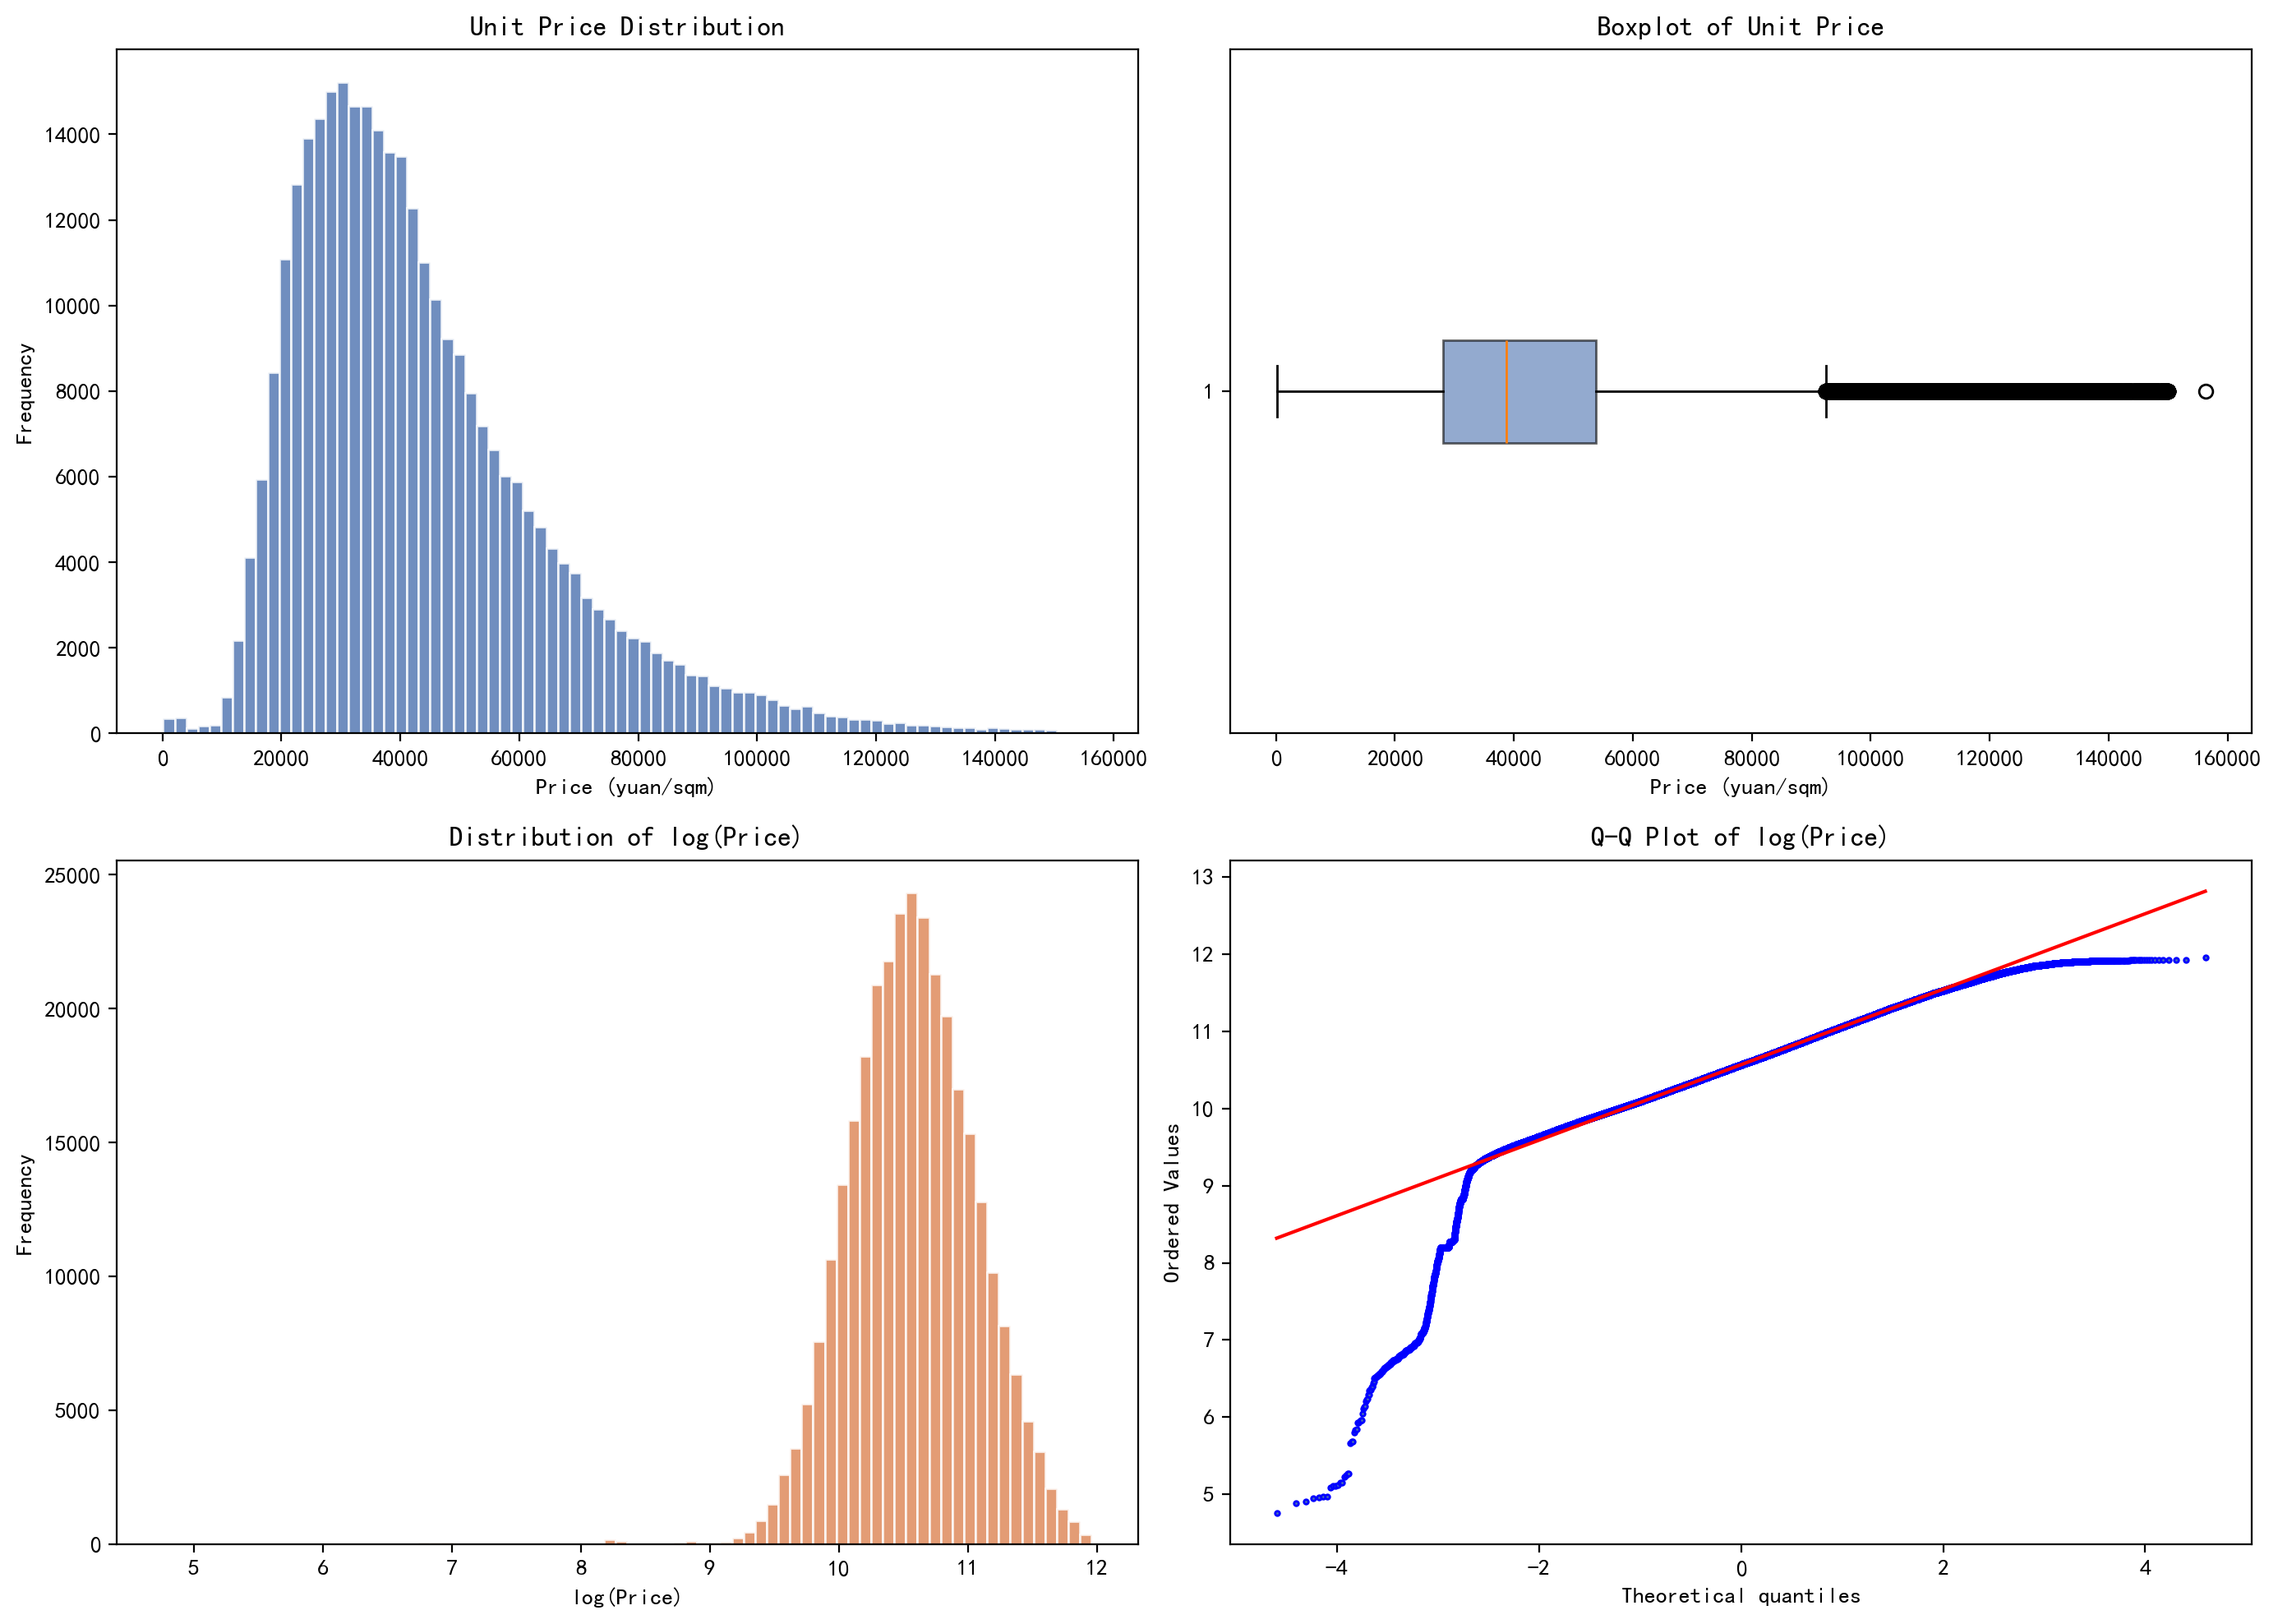
\includegraphics[width=0.75\textwidth]{01_eda/price_distribution.png}
\caption{价格分布与对数变换对比}
\label{fig:price_dist}
\end{figure}

\subsection{相关性分析}

相关性热力图显示，\textit{livingRoom}与
\textit{square}之间存在强正相关（$r=0.72$），验证了前文对多重共线性的预警。
在剔除数据泄露变量后，与价格相关性最高的变量依次为经纬度和面积、
建造年份。区域虚拟变量与价格的相关性呈现清晰的空间梯度，与北京市中心高、外围低
的房价格局一致。

\begin{figure}[H]
\centering
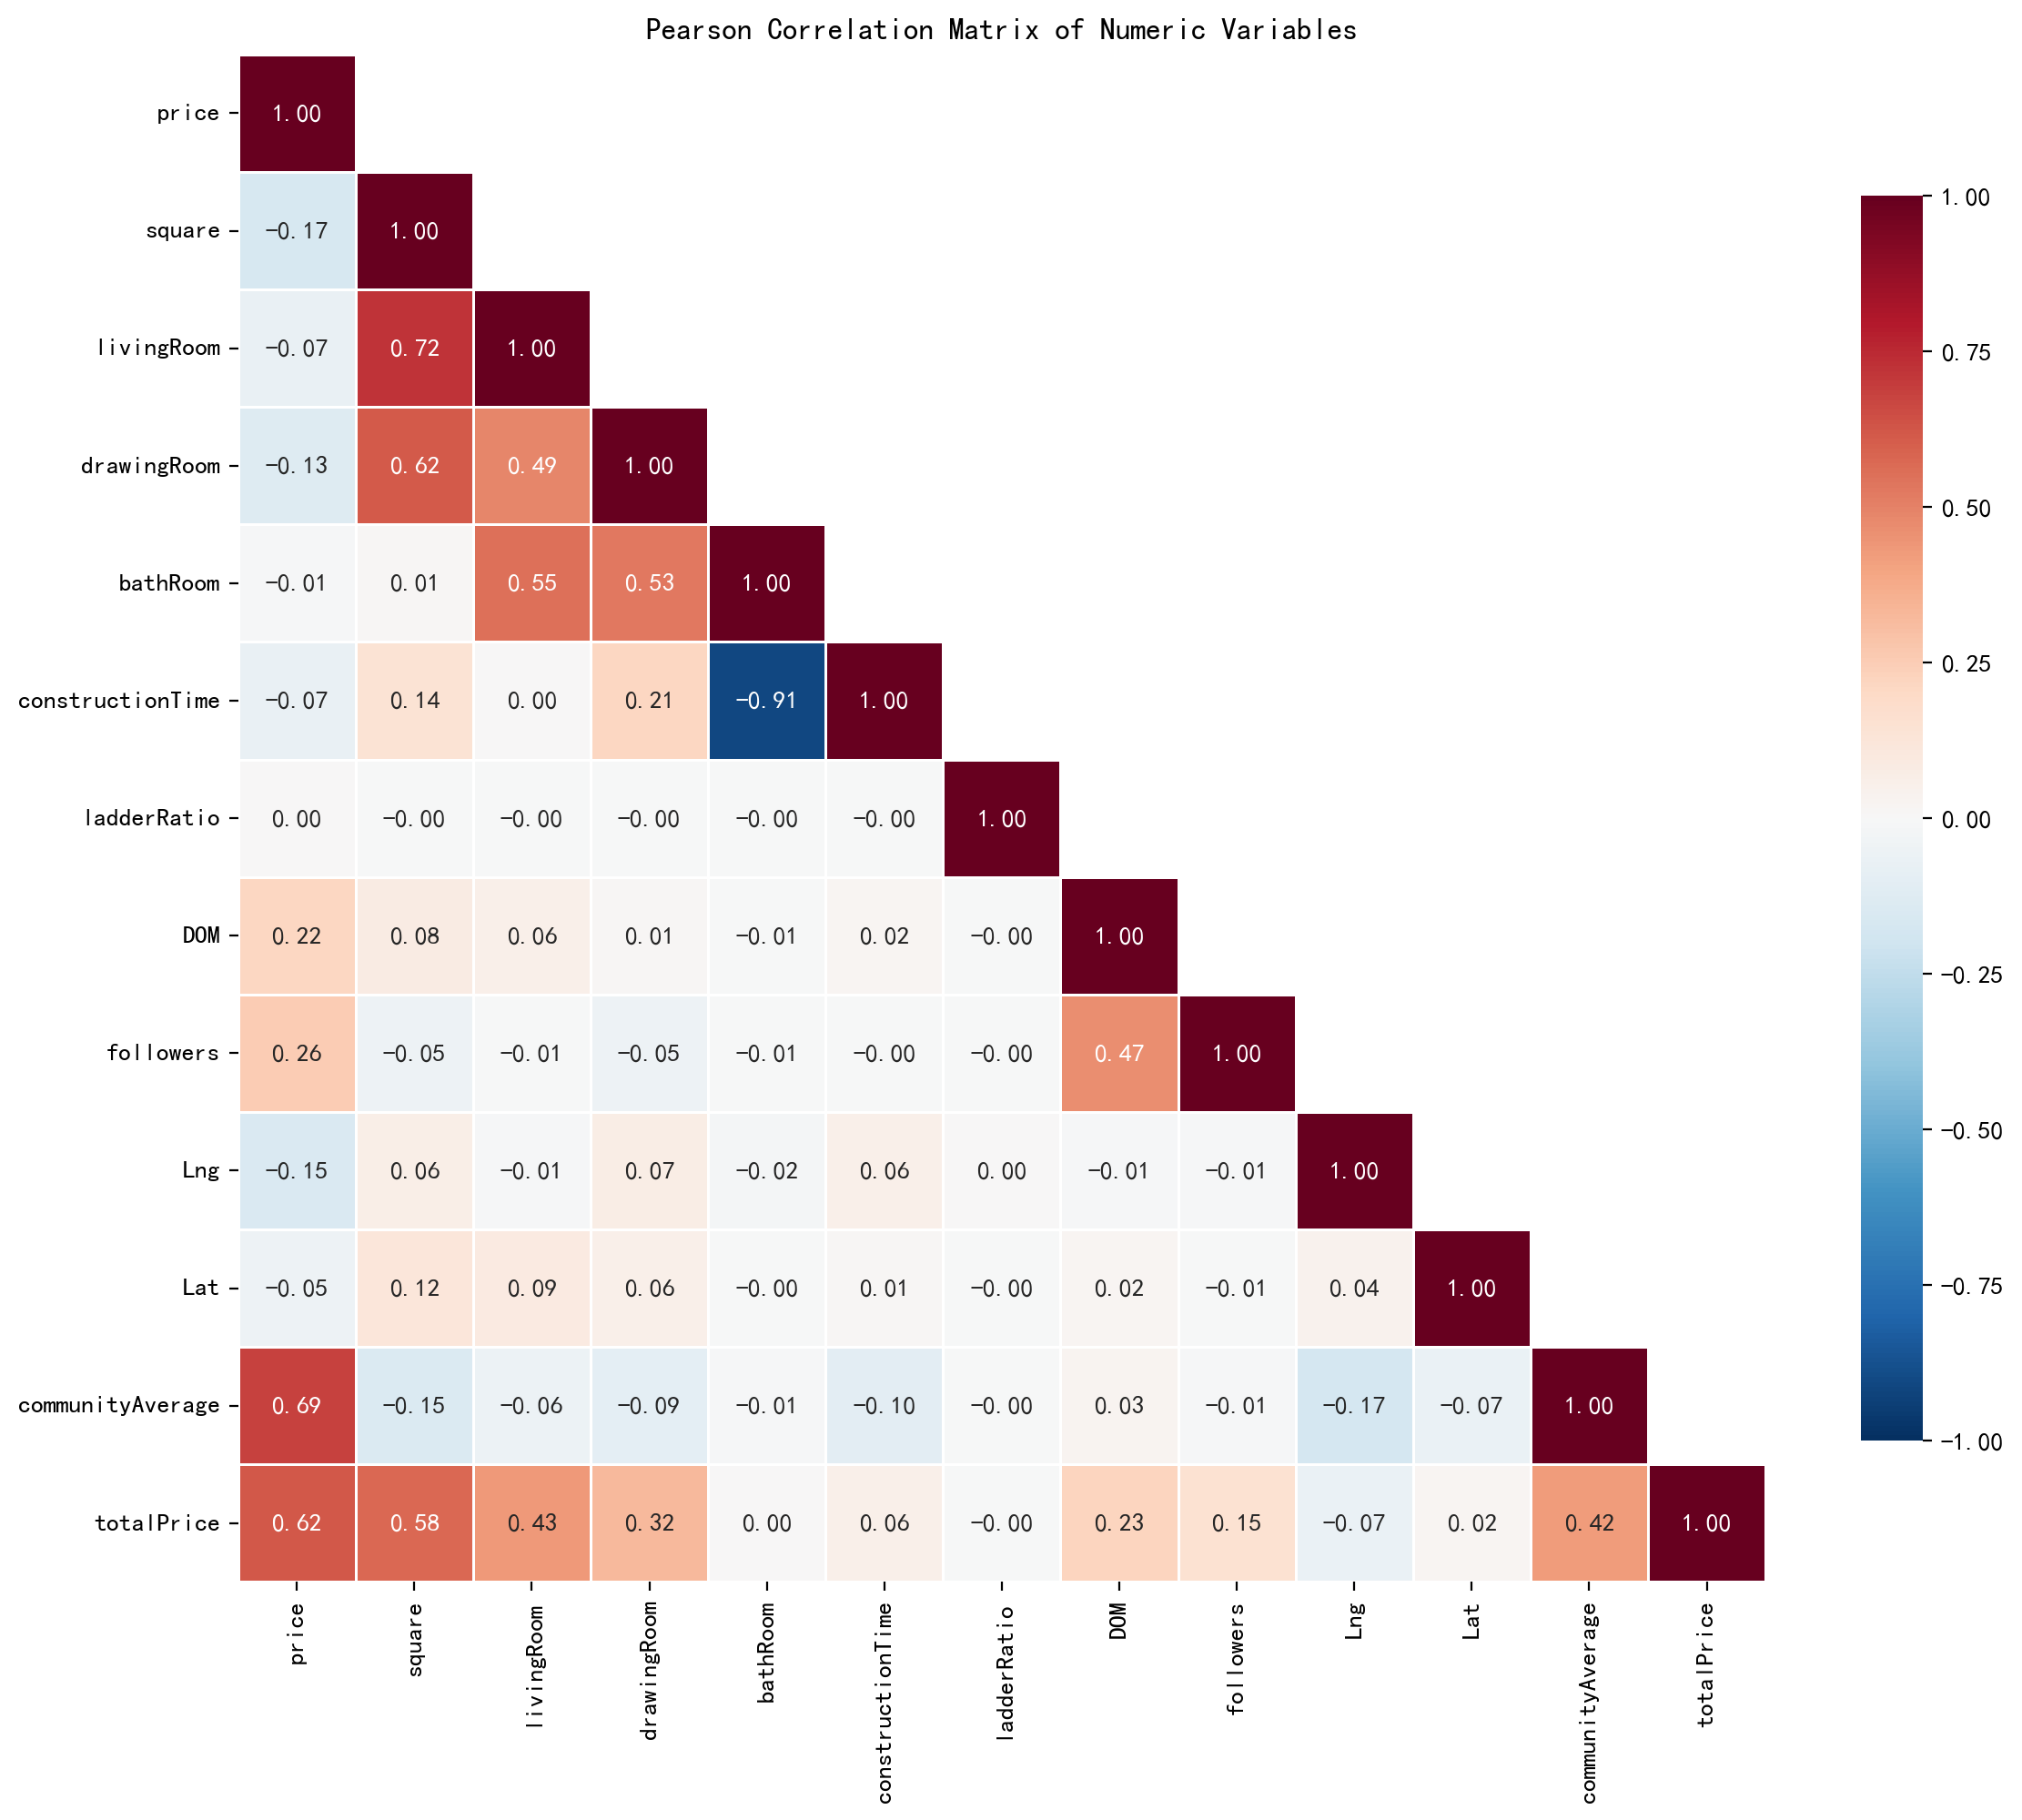
\includegraphics[width=0.7\textwidth]{01_eda/correlation_heatmap.png}
\caption{相关性热力图}
\label{fig:correlation}
\end{figure}

\subsection{地理分布与空间自相关}

房价的地理分布呈现典型的单中心城市空间模型特征。
散点图中的颜色梯度从市中心向外围呈辐射状
衰减，高价位房源高度集中于东城区、西城区和朝阳区核心地段，远郊区价格显著偏低。
各区域均价差异明显，中心城区均价最高，远郊区域均价较低，价差达三到四倍。

\begin{figure}[H]
\centering
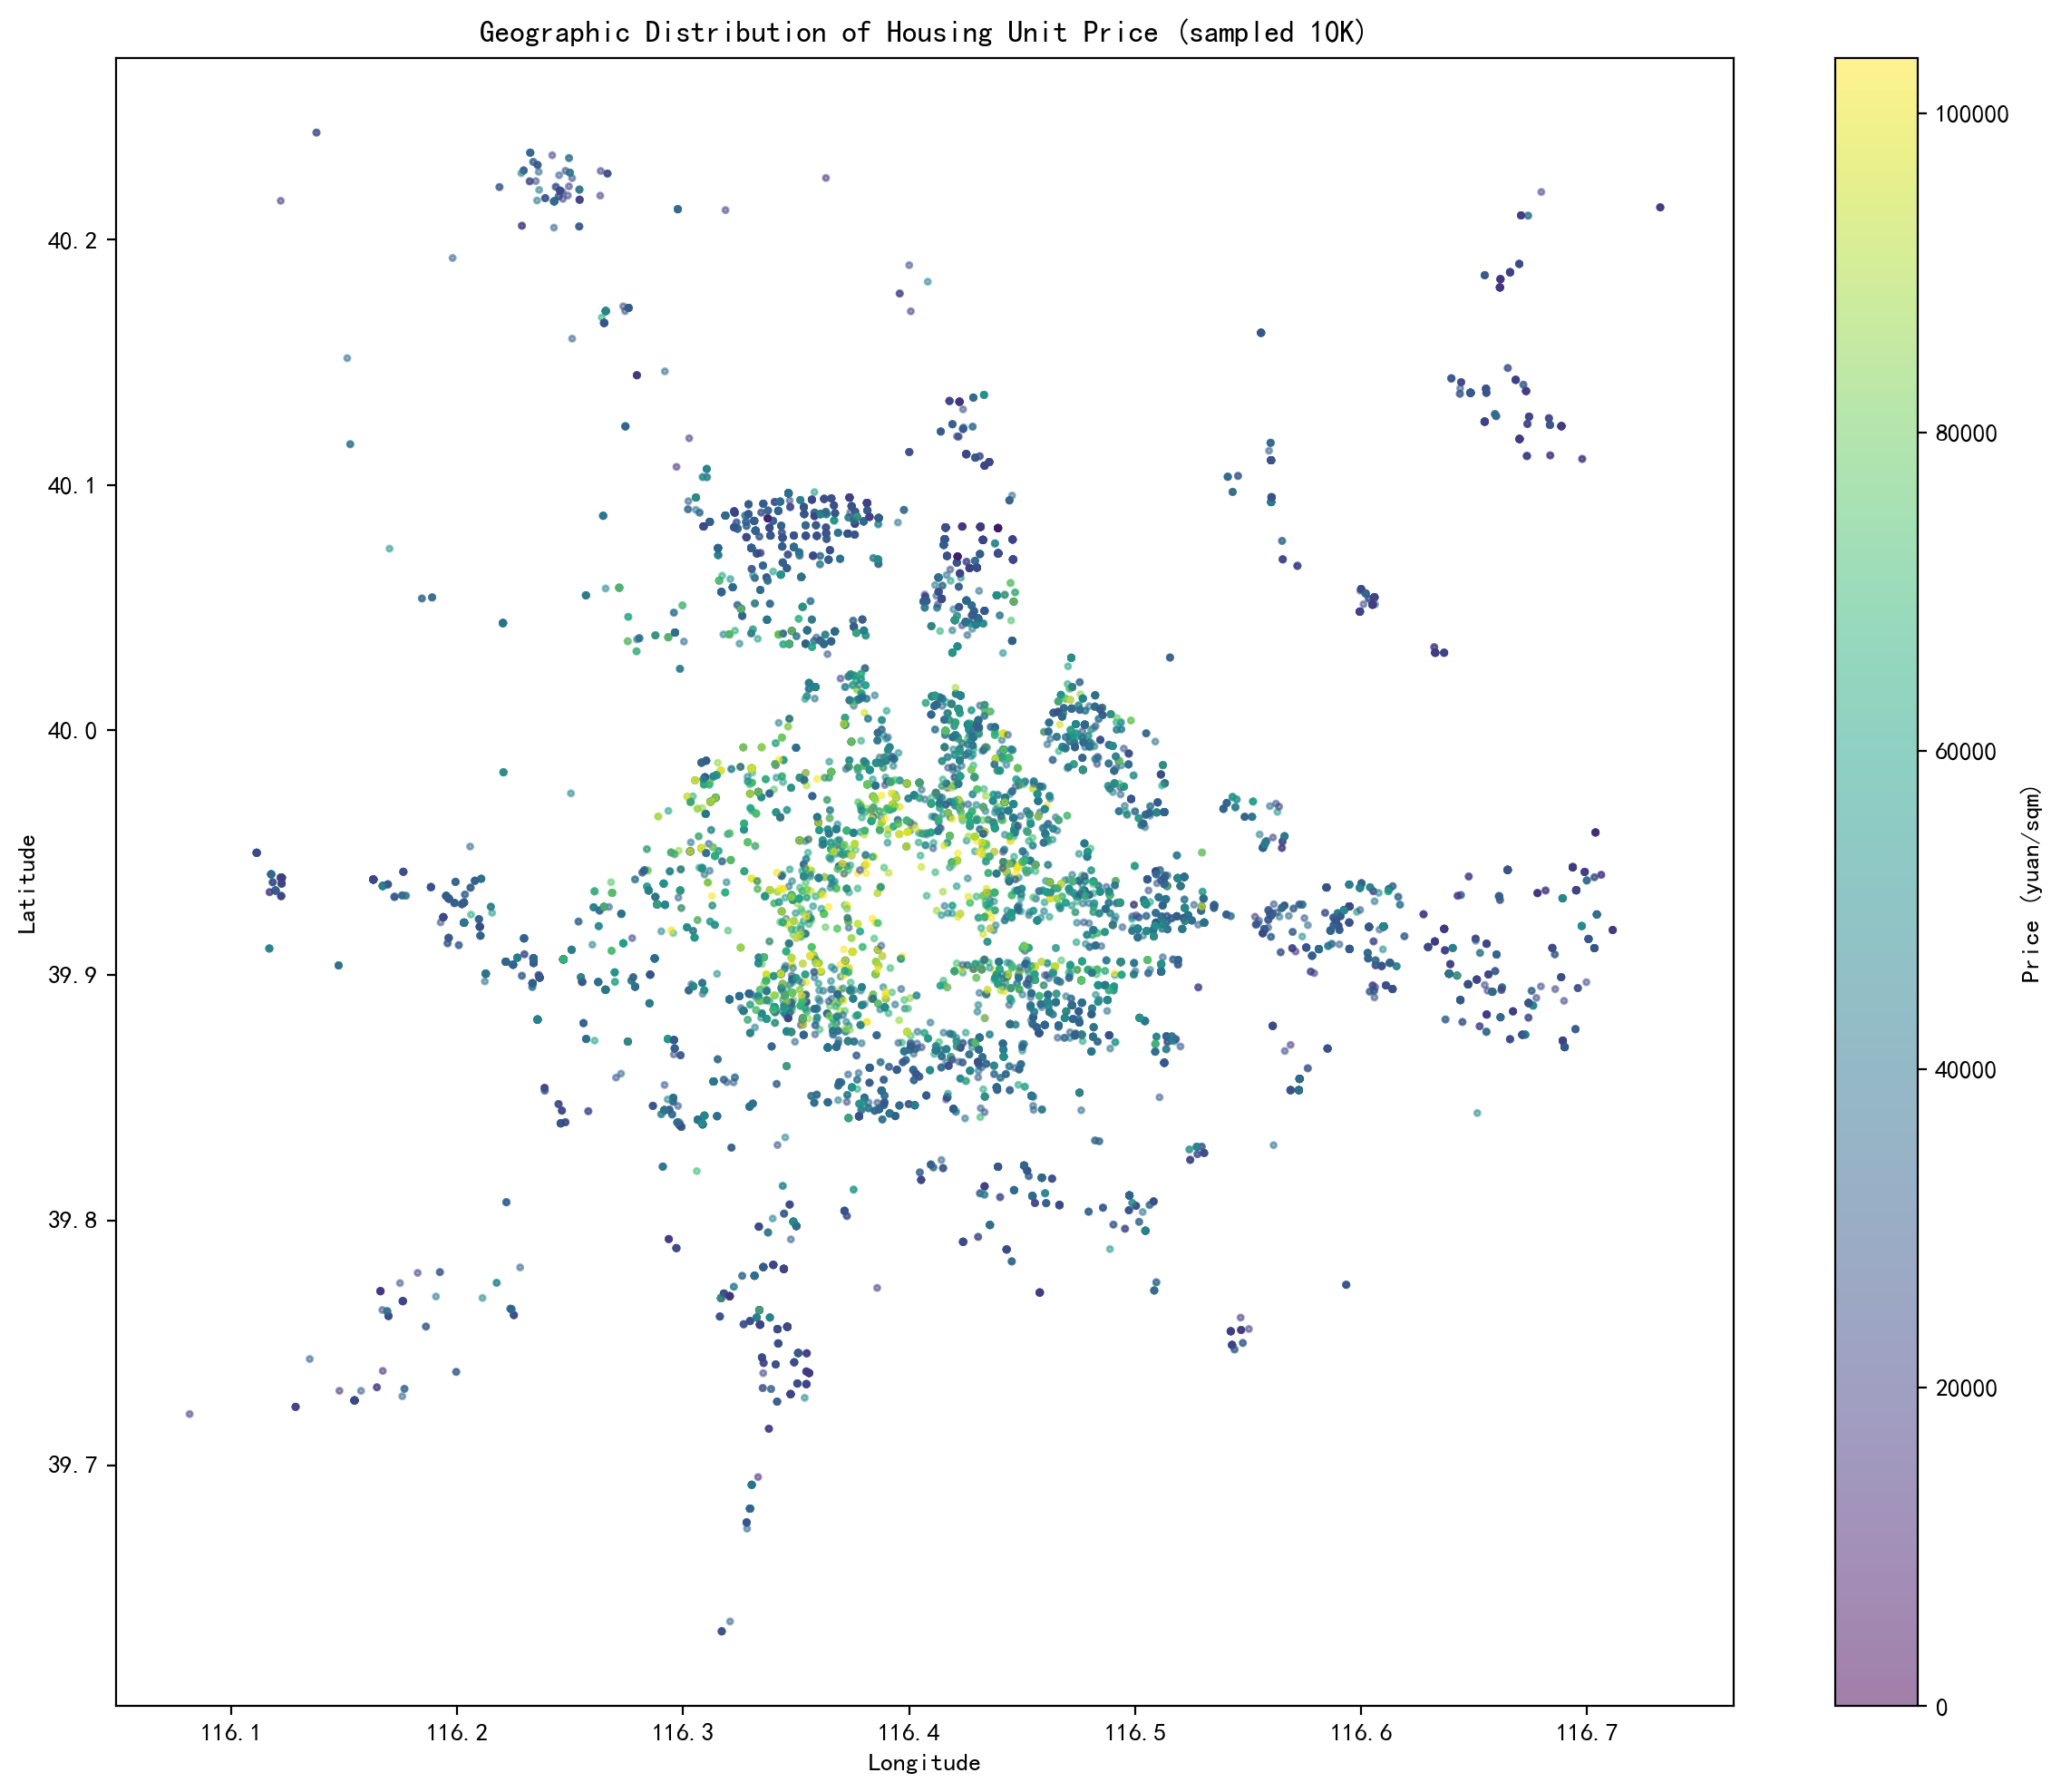
\includegraphics[width=0.7\textwidth]{01_eda/geo_price_scatter.png}
\caption{房价地理分布散点图}
\label{fig:geo}
\end{figure}

这种明显的空间聚集性意味着样本观测之间可能并非独立同分布——邻近房源的不可观测
特征往往相似，导致误差项在空间上相关。从空间计量经济学的视角，需要区分两种情形：
若真实的数据生成过程为空间误差模型，即空间相关性来源于误差项的聚类结构，则OLS
估计量仍然保持一致性和无偏性，但标准误有偏、估计效率降低；若真实过程为空间自回归
模型，即房价直接受邻近房源价格影响，则遗漏空间滞后项将导致遗漏变量偏误，估计量
有偏且不一致。本文的OLS框架尚未直接处理上述空间依赖性，但在此指出这一区分对于
理解空间效应的估计后果具有重要意义。

\subsection{价格时间趋势}

2011至2017年间，北京二手房均价总体呈上升趋势，但时间路径呈现明显的非线性特征。
2011至2015年初为平缓上涨阶段，2015年下半年至2017年进入加速上涨阶段，均价从约
4万元/m$^{2}$跃升至约7万元/m$^{2}$。这一趋势与同期的货币政策宽松、房地产去库存
政策以及2016年「9·30新政」前的市场预期升温密切相关。

\begin{figure}[H]
\centering
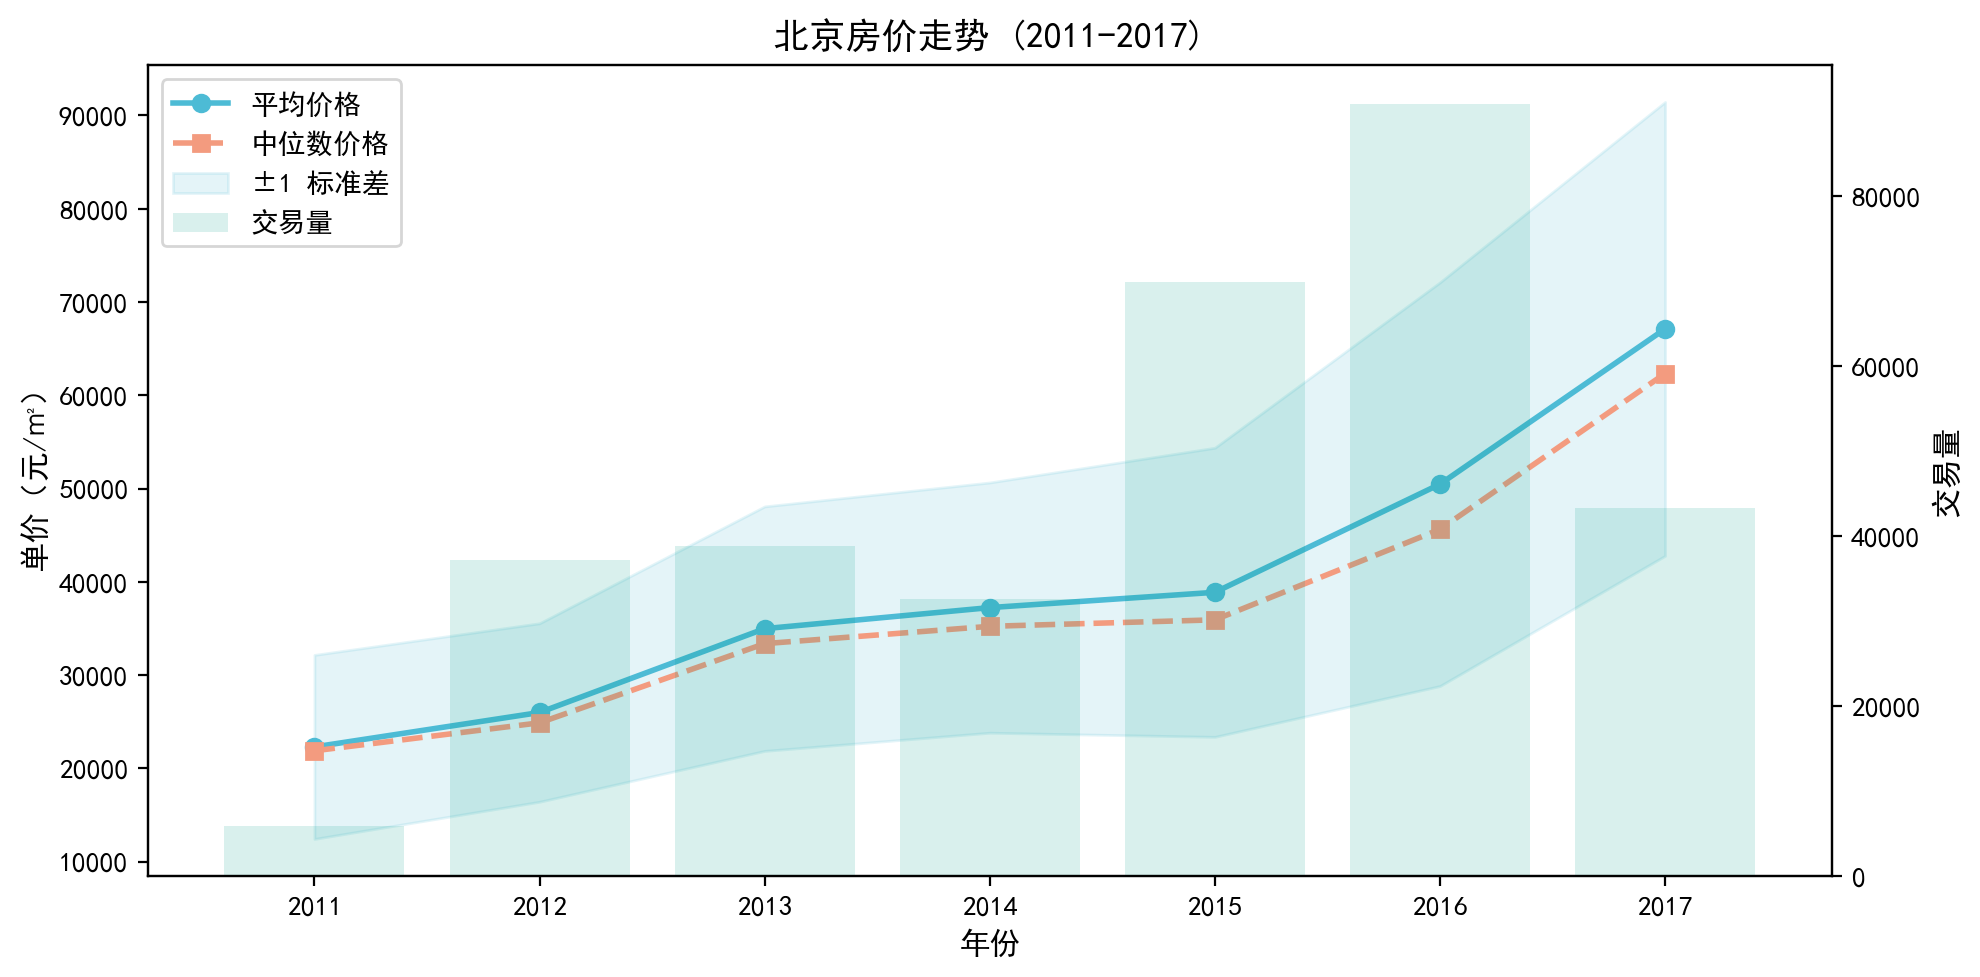
\includegraphics[width=0.7\textwidth]{01_eda/price_trend_by_year.png}
\caption{分年度价格趋势}
\label{fig:price_trend}
\end{figure}

这一发现具有重要的计量含义。在早期版本的模型中，\textit{trade\_year}被作为连续
线性变量纳入回归，实质上施加了「年度价格增幅恒定」的约束，这显然不符合数据特征。
在本文的最终模型设定中，\textit{trade\_year}已被替换为年份虚拟变量，同时纳入
月度虚拟变量控制季节性，让数据自行估计每年的基准价格水平。
后文表~\ref{tab:model_comparison}~显示，年份虚拟变量的系数从2012年的约$+0.15$
逐渐递增至2017年的约$+1.15$，年与年之间的增幅并不相等——2015年后的系数跳跃
明显更大，与EDA观察到的趋势转折完全一致。这验证了时间固定效应设定的合理性。

% ──────────────────────────────
%  四、模型设定与变量选择
% ──────────────────────────────
\section{模型设定与变量选择}

\subsection{基准回归模型}

本研究在特征价格模型框架下，设定包含时间和区域双向固定效应的半对数回归方程作为
基准模型：

\begin{equation}\label{eq:baseline}
\log(\text{Price}_{it}) = \beta_0 + \bm{X}_{it}'\bm{\beta} + \gamma_t + \delta_k + \varepsilon_{it}
\end{equation}

其中 $\log(\text{Price}_{it})$ 为第 $i$ 条交易在第 $t$ 期的对数价格；
$\bm{X}_{it}$ 包含连续型房屋和区位特征。$\gamma_t$ 为时间固定效应，由年度虚拟
变量（\textit{trade\_year\_2012}至\textit{trade\_year\_2017}，以2011年为基期）
和月度虚拟变量（\textit{trade\_month\_2}至\textit{trade\_month\_12}，以1月为
基期）共同实现；$\delta_k$ 为区域固定效应。

该设定的关键优势在于不施加年度价格增幅恒定的线性约束，允许数据自行估计每年的
基准价格水平。第三节的探索性分析已表明2011--2017年房价趋势呈明显非线性特征——
2015年前平缓上涨、2015年后加速攀升，因此 $\gamma_t$ 的灵活设定远优于线性趋势变量。
月度虚拟变量则进一步控制季节性波动。

为探索空间和房屋属性变量的非线性边际效应，对5个关键连续变量构造多项式扩展模型：

\begin{equation}\label{eq:poly}
\log(\text{Price}) = \beta_0 + \bm{X}'\bm{\beta} + \bm{Z}'\bm{\gamma} + \operatorname{vec}(\bm{Z} \otimes \bm{Z})'\bm{\theta} + \varepsilon
\end{equation}

其中 $\bm{Z}$ 为5个关键连续变量（\textit{dist\_center}、\textit{Lat}、
\textit{Lng}、\textit{ladderRatio}、\textit{DOM}）组成的向量。经度和纬度参与
扩展以捕捉空间曲面的弯曲，梯户比和挂牌天数参与扩展以允许边际效应递减。
\textit{trade\_year}不再参与多项式扩展，因为时间固定效应已通过年度虚拟变量灵活
捕捉了非线性的时间趋势。$\bm{Z} \otimes \bm{Z}$ 包含所有二次项和两两交互项。
该设定允许关键变量存在非线性边际效应，但代价是引入严重的多重共线性（见第五
章）。上述线性基准模型（带有时间-区域双向固定效应）是本文进行经济推断的主要依据，
而多项式模型主要用于对比和展示非线性扩展的代价。

\subsection{变量选择的共识策略}

为在高维特征空间（64个特征，含时间固定效应）中识别最重要的预测变量，本研究综合
运用三种方法：基于AIC的向前选择、基于AIC的向后剔除，以及LASSO正则化路径。
采用共识策略确定最终变量集，以增强变量选择的稳健性。

变量选择结果如下：全部64个特征中，29个被三种方法一致选中，30个被两种
方法选中，4个仅被一种方法选中，1个未被任何方法选中。最终共识变量集
包含59个变量。三种方法的一致性程度较高。被一致选中的重要变量包括经纬度、
距市中心距离、梯户比、有无电梯、临近地铁、
建筑面积对数及大部分区域虚拟变量。
值得注意的是，年份虚拟变量和多数月份虚拟变量同样被全票选中，验证了时间固定效应
纳入模型的必要性。

\subsubsection{LASSO 正则化与惩罚力度问题}

\begin{figure}[H]
\centering
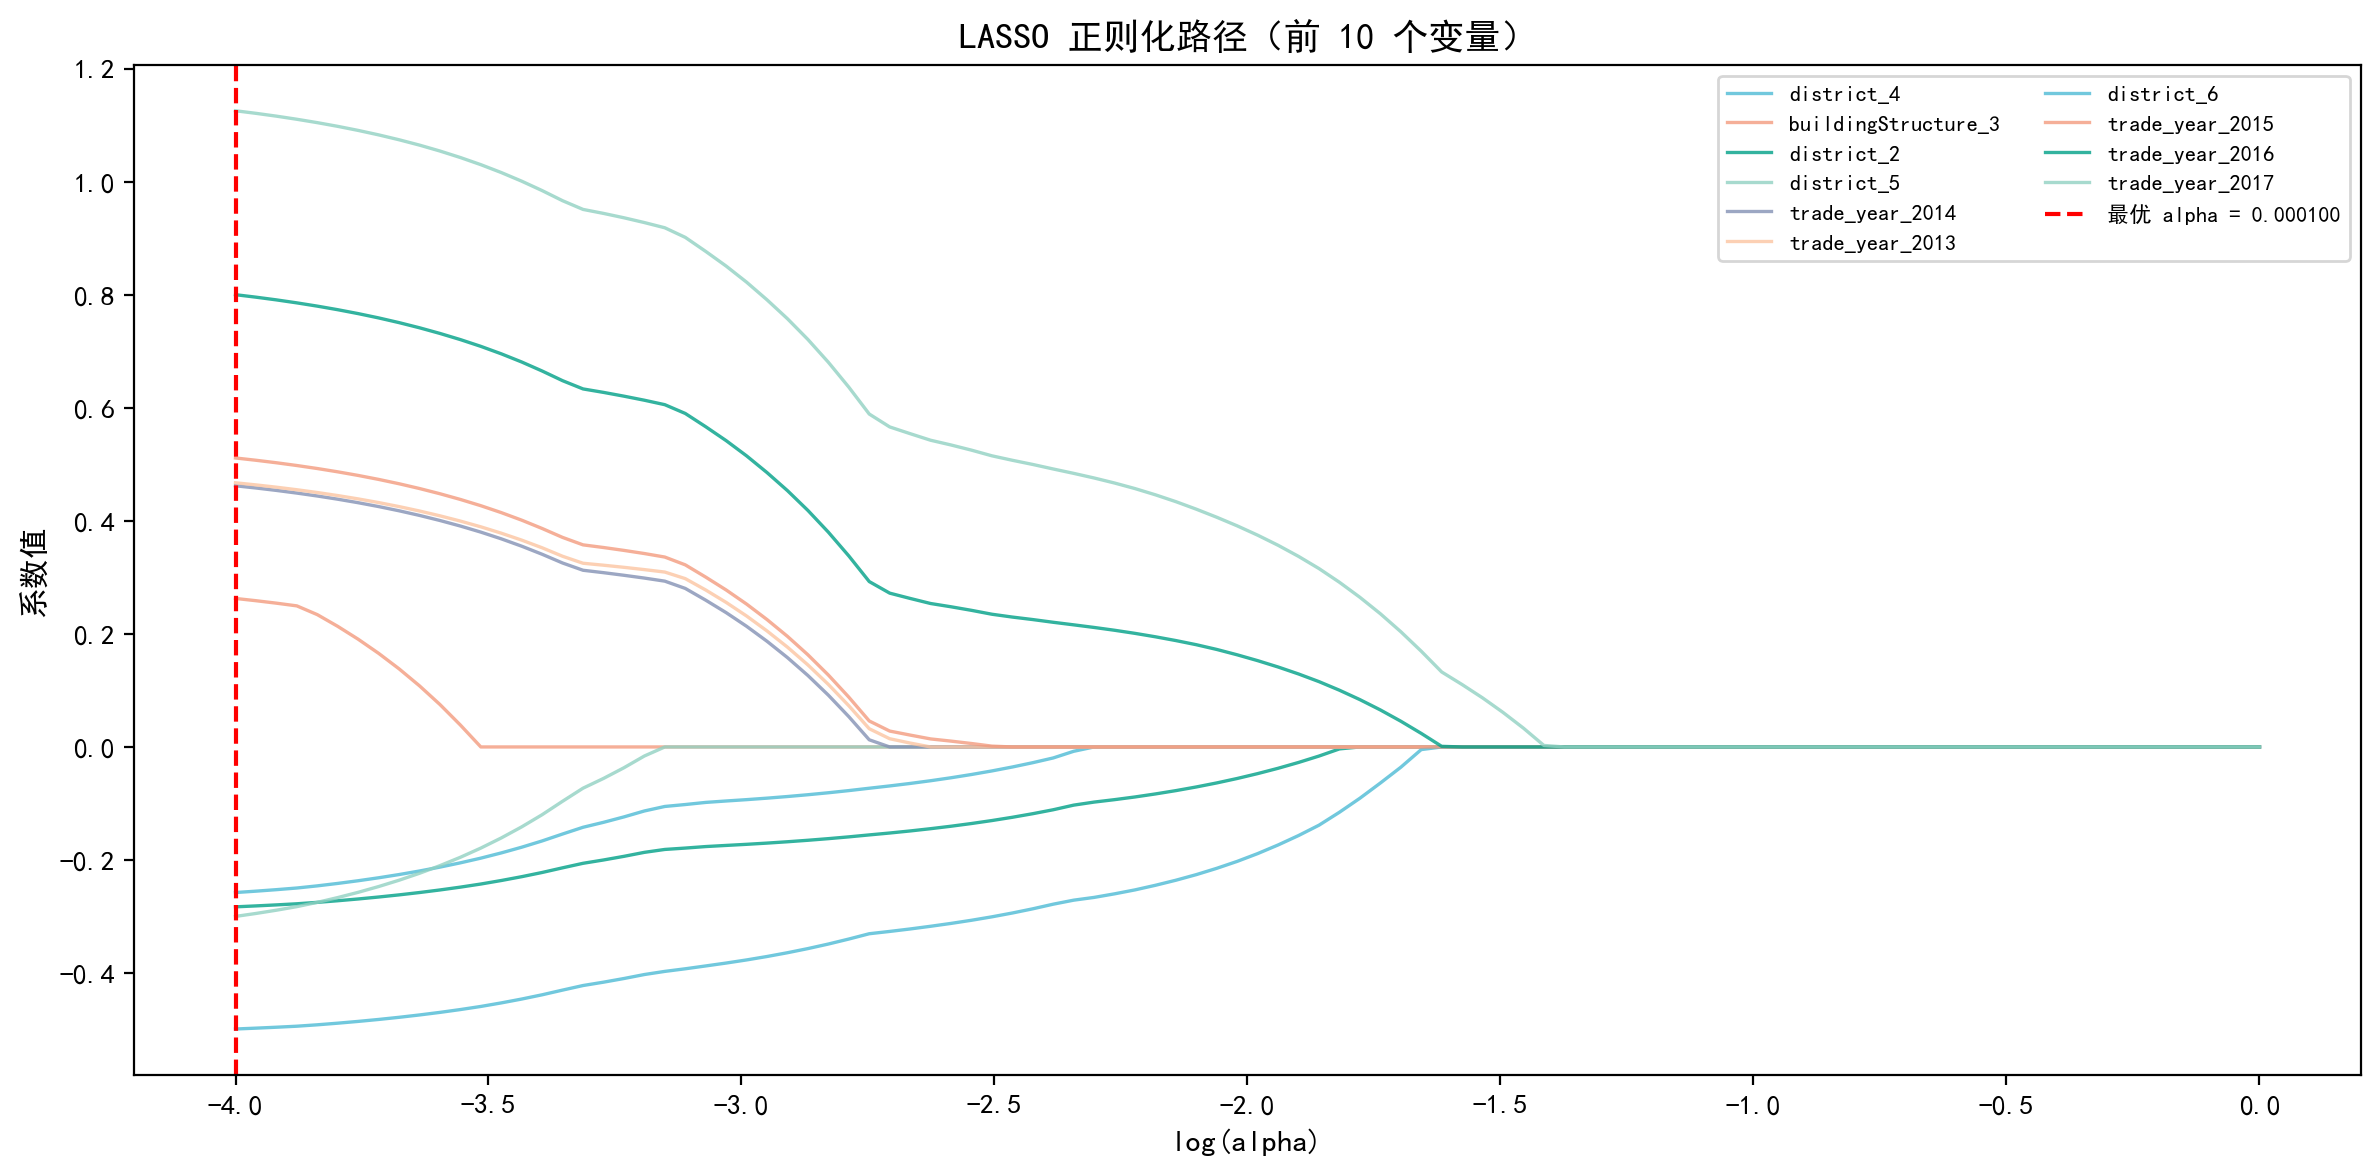
\includegraphics[width=0.75\textwidth]{03_selection/lasso_path.png}
\caption{LASSO正则化路径}
\label{fig:lasso}
\end{figure}

LASSO交叉验证选择的最优惩罚参数为 $\alpha=0.0001$，恰好位于搜索网格
$[10^{-4}, 10^{0}]$ 的下界。图~\ref{fig:lasso}~显示，模型在此参数下保留了
60/64个非零系数，惩罚力度极为微弱。将搜索网格向下扩展至
$10^{-5}$ 后，最优 $\alpha$ 仍然落在新的下界，表明这一结果并非网格设定问题所导致。

这一现象的数据解释是：64个候选特征中绝大多数都与房价存在统计上显著的关联，强预测
信号在特征空间中广泛分布，LASSO无法通过L1惩罚将有效信号压缩为零。这与真实模型
稀疏的隐含前提相悖——住房价格通常受众多微效因素共同影响。因此LASSO在本应用中
本质上退化为了普通OLS，这也解释了为何在后文的模型比较中二者的预测表现几乎完全一致。

% ──────────────────────────────
%  五、模型诊断
% ──────────────────────────────
\section{模型诊断}

基于全变量OLS模型（子样本20\,000行），对经典线性回归的假设条件进行系统检验。

\subsection{诊断检验结果}

\begin{table}[H]
\centering
\caption{模型诊断结果汇总}
\label{tab:diagnostics}
\begin{tabular}{lp{10cm}}
\toprule
检验项目 & 结果 \\
\midrule
VIF $>$ 10 变量数 & 9个：buildingStructure系列、square、log\_square、trade\_year\_2016/2015/2017 \\
最大VIF（不含常数项） & 492.4（buildingStructure\_6） \\
条件数 & $4.59\times10^{5}$（较原模型 $7.84\times10^{6}$ 大幅改善） \\
Breusch-Pagan检验 & LM=957.6，$p=1.8\times10^{-159}$，拒绝同方差 \\
Goldfeld-Quandt检验 & $F=0.979$，$p=0.857$，不拒绝同方差 \\
Durbin-Watson统计量 & 1.966，无自相关 \\
Cook's D异常点比例 & 4.74\%（947/20\,000）超过阈值 \\
HC3下显著性改变量 & 1个变量（fiveYearsProperty\_1.0） \\
\bottomrule
\end{tabular}
\end{table}

\subsection{多重共线性讨论}

表~\ref{tab:diagnostics}~报告了VIF诊断结果。\textit{buildingStructure\_6}
和\textit{buildingStructure\_2}存在严重的多重共线性。
这与\textit{buildingStructure}变量的类别分布密切相关：某些结构类别的占比极低，
导致相应的虚拟变量与其他结构类别之间呈现近乎完全的线性关系。此外，
\textit{square}和\textit{log\_square}之间的高度相关性也反映了
面积变量在对数-线性变换后的共线性问题。部分年份虚拟变量的VIF超过10，
这是以2011年为高基期、多年度同时纳入模型时的自然结果。

对于以OLS为基础的统计论文，9个VIF大于10的变量虽然不影响模型的整体预测能力，但
会膨胀个体系数的标准误、降低估计精度。值得注意的是，加入时间固定效应后条件数从
$7.84\times10^{6}$降至$4.59\times10^{5}$，这是因为原模型中的
\textit{trade\_year}连续变量与其平方项之间存在大量共线性，被年份虚拟变量替代后
这一来源得到消除。在OLS与多项式组合模型中，多重共线性问题因高阶项的加入而显著
加剧，详见第~\ref{sec:poly_inflation}~节。

\subsection{异方差与残差分析}

Breusch-Pagan检验在1\%水平上显著拒绝同方差假设，而Goldfeld-Quandt检验未能检测到
异方差。两个检验结论的不一致根源在于检验功效和敏感性的差异：BP检验对一般形式的
异方差均敏感，而GQ检验仅对排序后单调变化的方差敏感。残差诊断图显示，当拟合值增大
时残差幅度呈现扩散趋势，这一漏斗状模式支持BP检验的结论，即样本中存在不可忽略的
异方差。

\begin{figure}[H]
\centering
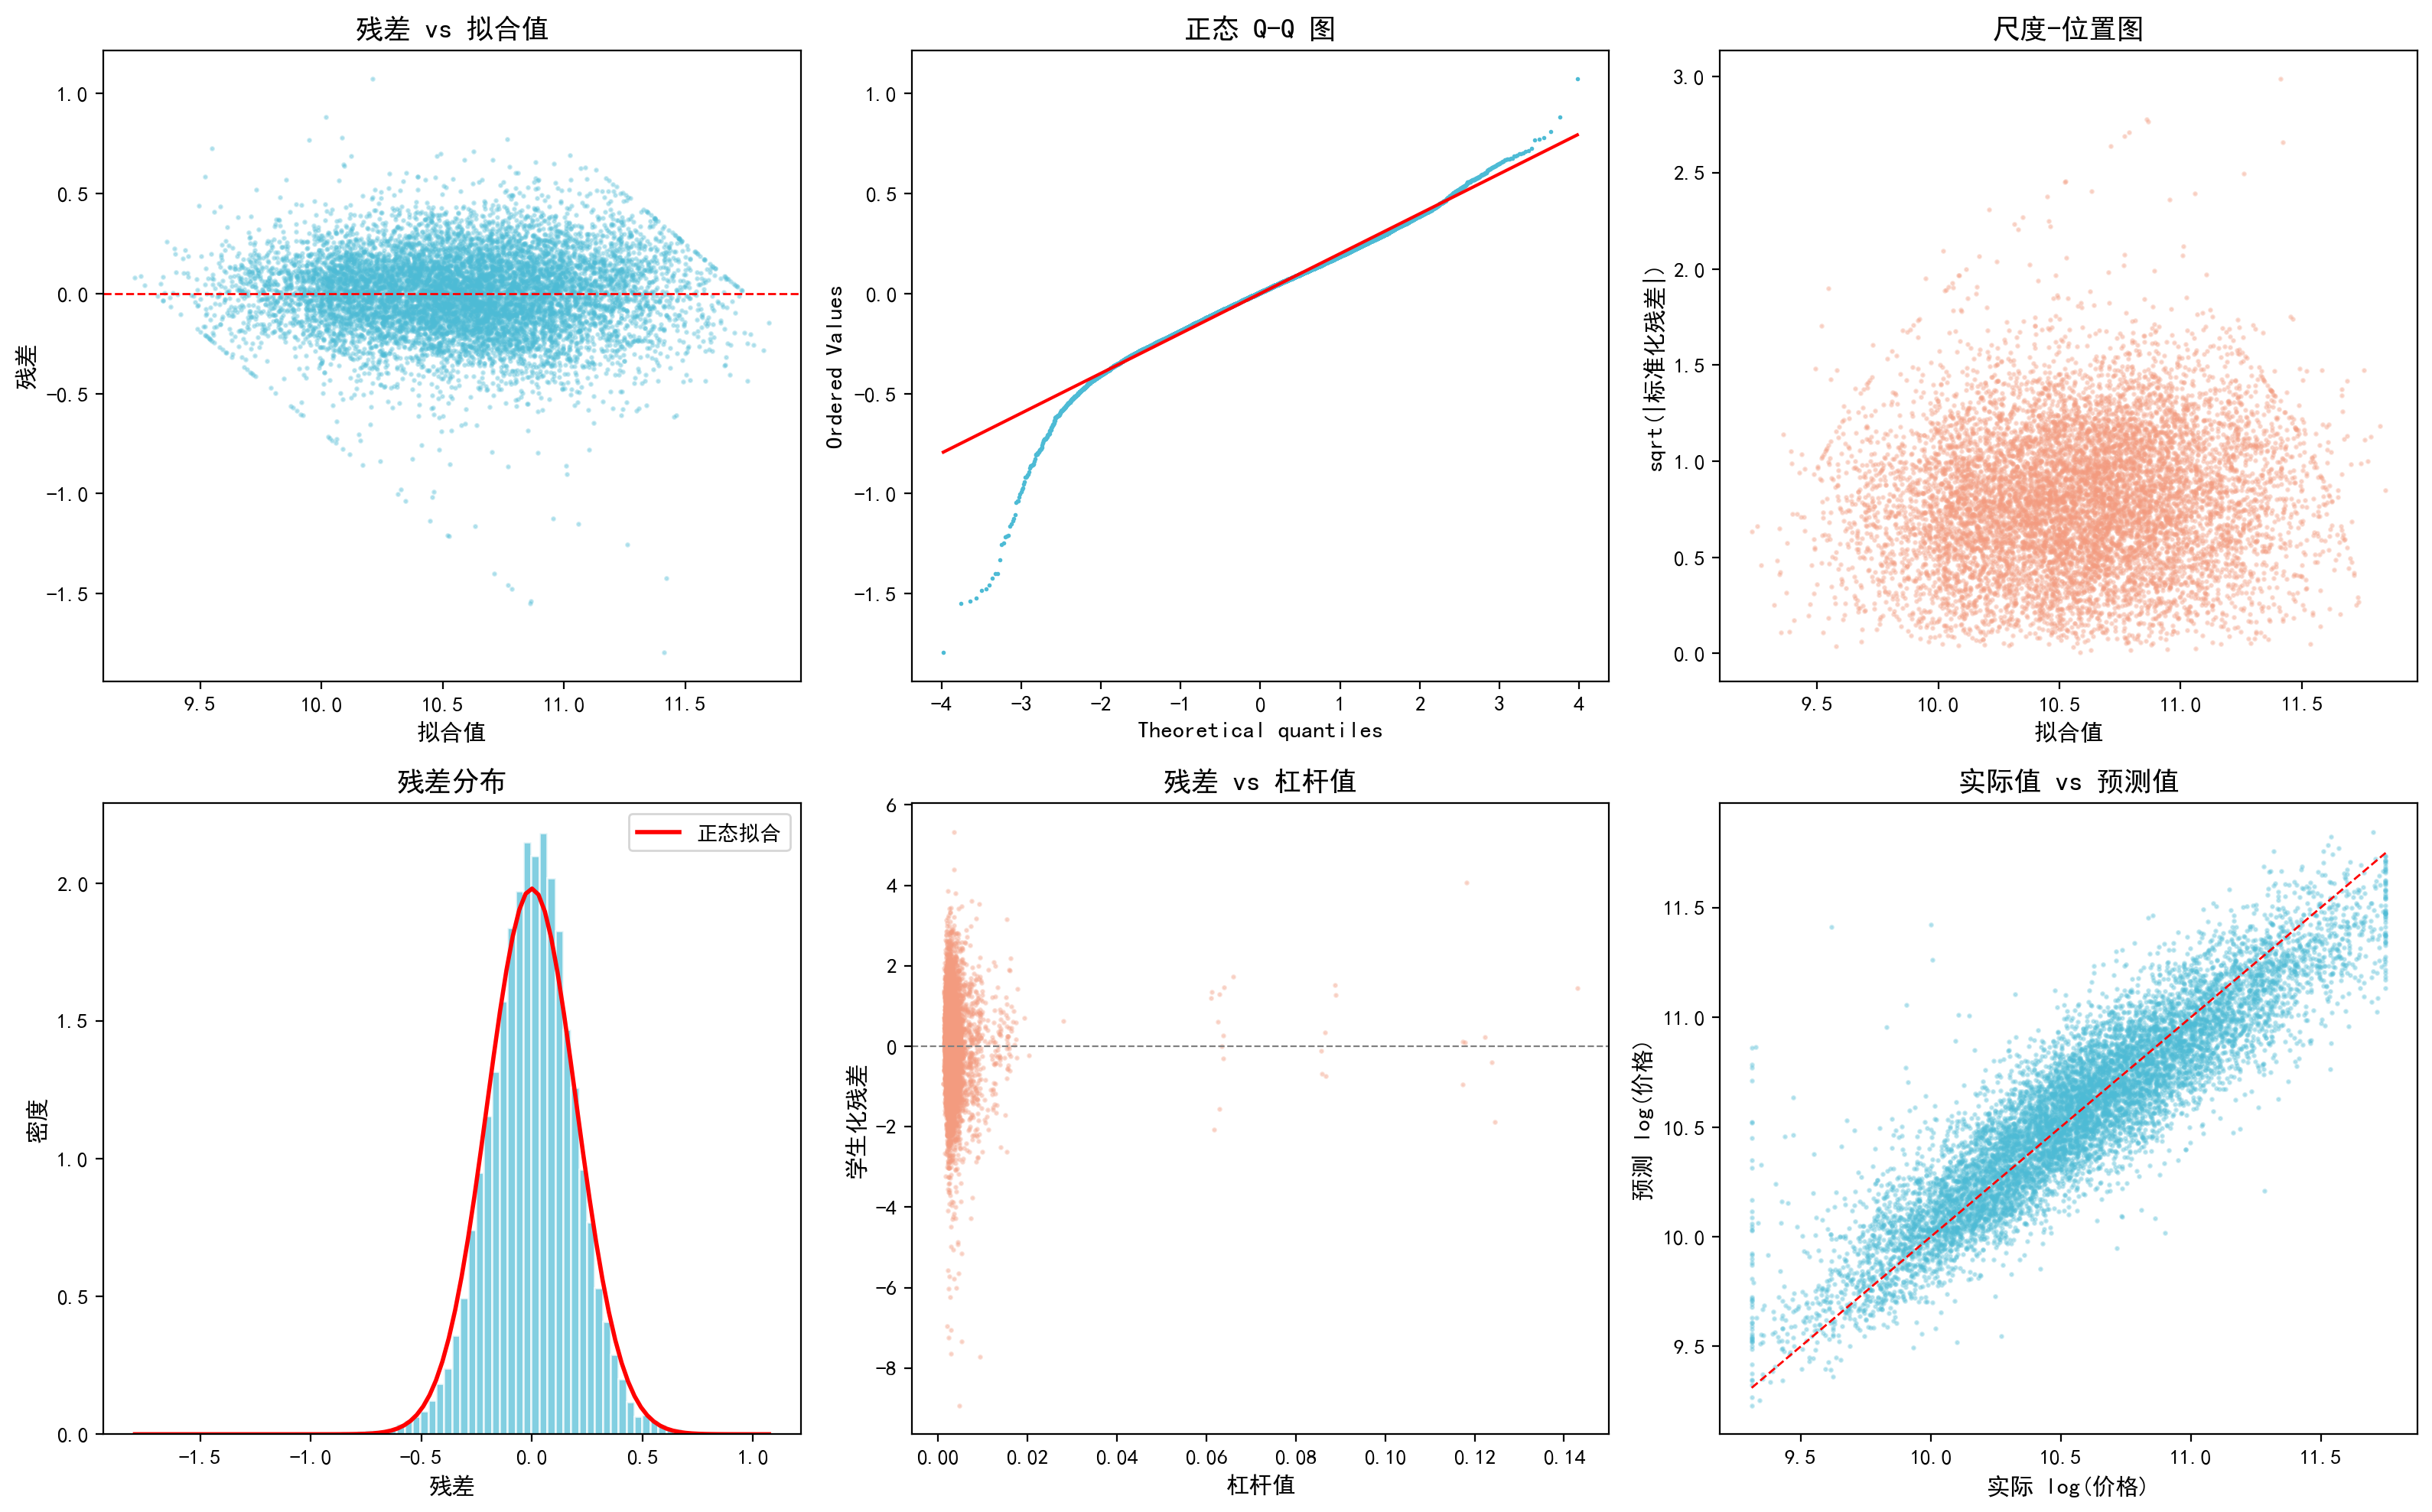
\includegraphics[width=0.75\textwidth]{04_diagnostics/residual_diagnostics.png}
\caption{残差诊断图（左上：残差vs拟合值；右上：尺度-位置图；左下：Q-Q图）}
\label{fig:residual}
\end{figure}

\subsection{稳健标准误}

采用HC3稳健标准误对OLS系数进行校正。结果表明校正后仅一个变量
\textit{fiveYearsProperty\_1.0}的显著性判断发生改变，从$p=0.048$变为
$p=0.053$，略超5\%阈值。这一结果优于原模型，说明加入
时间固定效应后异方差对推断的干扰进一步减弱。因此，HC3稳健标准误的使用主要作为
学术严谨性的必要组成部分，而非因为实质性改变了结论。

截面数据的异方差在真实世界中是常态而非异常。本研究从事前和事后两个层面确保了推断
的可靠性。事前，半对数设定将绝对差异转化为相对差异，从数据变换的根源上缓解了方差
随价格水平递增的趋势；事后，HC3稳健协方差矩阵的修正进一步消除了异方差对标准误
估计的干扰。因此，即便Breusch-Pagan检验明确拒绝了同方差假设，核心变量边际效应
的推断结果仍然是稳健且可靠的。

% ──────────────────────────────
%  六、模型比较与结果解释
% ──────────────────────────────
\section{模型比较与结果解释}

本研究比较了六种回归模型在测试集上的表现：OLS全变量模型、Ridge回归、LASSO回归、
OLS共识筛选变量模型、OLS与交互项组合以及OLS与多项式组合。
其中\textit{trade\_year}因转为虚拟变量不再参与多项式扩展。

\subsection{预测表现比较}

各模型在测试集上的表现汇总于表~\ref{tab:model_comparison}。

\begin{table}[H]
\centering
\caption{测试集模型表现比较}
\label{tab:model_comparison}
\begin{tabular}{lcccr}
\toprule
模型 & $R^{2}$ & RMSE（元/m$^{2}$） & MAE（元/m$^{2}$） & AIC \\
\midrule
\textbf{OLS + 多项式}  & \textbf{0.8294} & \textbf{9\,411} & \textbf{6\,471} & \textbf{$-207\,770$} \\
OLS + 交互项          & 0.8218 & 9\,621 & 6\,631 & $-205\,038$ \\
OLS（全变量）         & 0.8185 & 9\,696 & 6\,703 & $-203\,859$ \\
Ridge（CV）           & 0.8185 & 9\,696 & 6\,703 & --- \\
OLS（筛选变量）       & 0.8184 & 9\,695 & 6\,703 & $-203\,867$ \\
LASSO（CV）           & 0.8180 & 9\,710 & 6\,713 & --- \\
\bottomrule
\end{tabular}
\end{table}

OLS与多项式组合模型在预测指标上表现最佳，$R^{2}=0.829$，RMSE为9\,411元/m$^{2}$，
较基准OLS提升约1.1个百分点。五折交叉验证结果与测试集一致，排除了
过拟合的可能。与旧版本模型相比，当前基准OLS
的$R^{2}$从0.786提升至0.818，RMSE从10\,428降至9\,696，
充分说明时间固定效应设定的有效性。然而，OLS与多项式模型之间的
$R^{2}$差距也从原来的1.9个百分点缩窄至1.1个百分点——这是因为时间固定效应已经
捕捉了部分原来多项式模型才能拟合的非线性时间趋势。

\subsection{核心变量的边际效应解释}

在评估模型时，本研究不仅关注预测精度，更重视核心变量边际效应的经济学含义。以下
基于共识变量OLS模型对关键变量进行半弹性解释。在对数-线性模型中，连续变量的系数
$\beta$的精确解释为：该变量增加一个单位时，响应变量变化
$100\times(e^{\beta}-1)\%$。当系数绝对值较小时，$\beta\times100\%$可作为近似。

首先考察空间因素的影响。距市中心距离的系数为$-2.681$，意味着距天安门每增加
0.01度，房价下降约2.65\%。以2017年北京二手房均价约6万元/m$^{2}$
计算，每远离市中心1公里，单价下降约1\,590元。这一效应在统计和经济意义上均高度
显著，印证了北京作为单中心城市的空间结构特征。

房屋建筑特征方面，有无电梯的系数为0.074，有电梯的房源比无电梯房源价格高出约
7.7\%。对于均价6万元/m$^{2}$的住宅，这一溢价约为4\,620元/m$^{2}$，折合到一套
80m$^{2}$的住房约为37万元。梯户比的系数为0.167，每增加0.1，房价上升约1.68\%，
反映了居住舒适度对房价的资本化效应。

交通便利性方面，临近地铁的系数为0.056，临近地铁的房源溢价约为5.8\%，体现了轨道
交通对住房价值的资本化效应。值得注意的是，这一效应在远郊区域可能更为显著，因为
远郊居民对轨道交通的依赖度高于中心城区。

\begin{figure}[H]
\centering
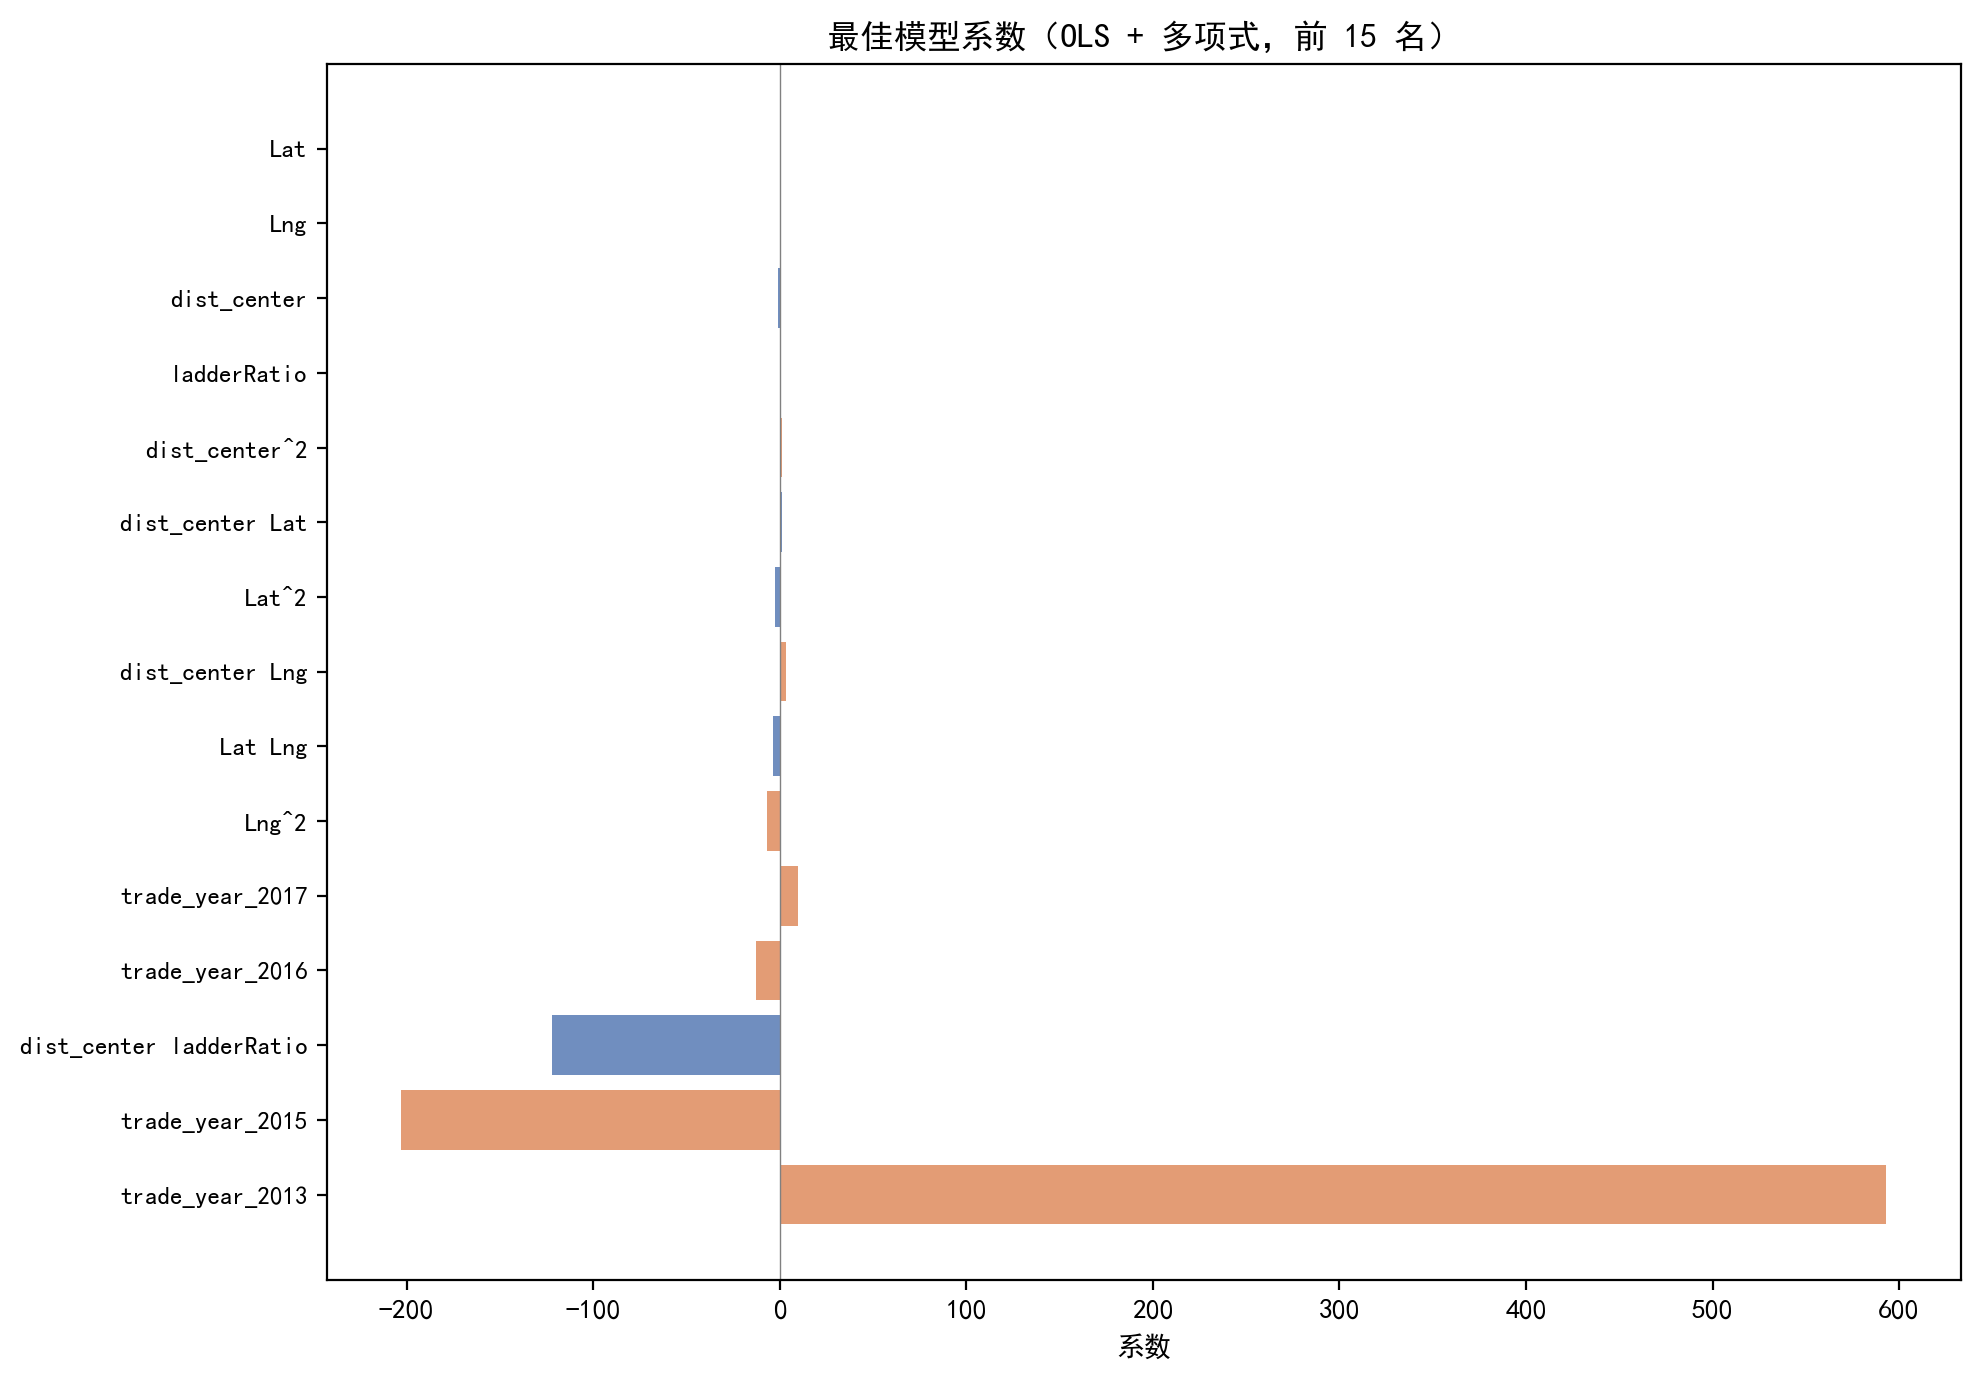
\includegraphics[width=0.75\textwidth]{05_comparison/best_model_coefficients.png}
\caption{最佳模型系数图（OLS+多项式，前15名）}
\label{fig:best_coef}
\end{figure}

\subsection{多项式模型的系数膨胀问题}
\label{sec:poly_inflation}

图~\ref{fig:best_coef}~展示了OLS与多项式组合模型中系数绝对值最大的15个变量。
部分区域虚拟变量的系数绝对值达到200至800的量级。由于响应变量为
$\log(\text{price})$，这意味着某区域的边际效应为$e^{200}$至$e^{800}$倍，在经济
意义上不再具有合理的解释力。

这一现象的根源在于：多项式扩展将5个关键变量（\textit{dist\_center}、\textit{Lat}、
\textit{Lng}、\textit{ladderRatio}、\textit{DOM}）扩展为20个二次项和交互项。
这些高阶项与已有的区域虚拟变量（\textit{district\_*}）之间存在严重的多重共线性——
区域本身就是地理空间的离散化表示，而经纬度的多项式组合是对同一空间的连续函数逼近。
二者高度相关导致正规方程（$\bm{X}'\bm{X}$）近乎奇异，条件数急剧恶化，回归系数
在理论上趋向无穷大，呈现出$\pm200$至$\pm800$的反常值。值得注意的是，虽然
\textit{trade\_year}已转为虚拟变量不再参与多项式扩展，但\textit{dist\_center}与
\textit{Lat}/\textit{Lng}之间的空间共线性仍然足以引发矩阵病态。

这一发现揭示了一个重要的方法论教训：线性回归模型在引入高阶多项式项后，虽然预测
精度有所提升，但其核心优势——系数可直接解释为边际效应——受到了根本性损害。当研究
目标是经济推断（inference）而非预测（prediction）时，简洁的主效应线性模型在设计
合理的固定效应设定下，通常是更为可靠的选择。

\subsection{时间趋势的进一步讨论}

在共识变量OLS模型中，以2011年为基期，年份虚拟变量的系数呈现清晰的递增模式：
\textit{trade\_year\_2012}（$+0.15$）、\textit{trade\_year\_2013}（$+0.48$）、
\textit{trade\_year\_2014}（$+0.49$）、\textit{trade\_year\_2015}（$+0.54$）、
\textit{trade\_year\_2016}（$+0.83$）和\textit{trade\_year\_2017}（$+1.15$）。
这一序列的特征在于：2013年较2012年有大幅跳跃（$+0.33$），而
2013--2015年间增幅相对平缓，年增约0.03至0.05，2015年后再次加速。
该模式与探索性数据分析中观察到的
「2011--2015年初平缓上涨、2015下半年后加速攀升」完全吻合。

在旧版模型中\textit{trade\_year}被作为连续线性变量（系数0.180），等效于为所有
年份施加了「年增幅约19.7\%」的单一系数，这必然低估2015年后的涨幅并高估
2011--2014年的涨幅。时间固定效应解决了这一问题，同时消解了旧版模型中需要依赖
\textit{trade\_year}$^{2}$项来部分捕捉非线性趋势的妥协。月度虚拟变量的系数也
从2月（$+0.046$）逐步递增至12月（$+0.190$），反映了一年内的季节性价格上升趋势。

% ──────────────────────────────
%  七、结论
% ──────────────────────────────
\section{结论}

\subsection{主要发现}

本研究通过特征价格模型框架和多种回归方法，对北京市住房价格的影响因素进行了系统的
实证分析，得到以下几方面主要发现。

第一，空间因素是解释房价差异的主导变量。距市中心距离、经纬度和区域虚拟变量具有
最强的解释力，北京市呈现单中心城市空间结构，距市中心每增加1公里，房价下降约
2.7\%，梯度效应显著。第二，时间因素具有非线性影响。年份虚拟变量系数从2012年的
$+0.15$逐步递增至2017年的$+1.15$，验证了2015年前后房价结构性加速的特征；
时间固定效应的设定显著优于连续的\textit{trade\_year}线性变量。第三，房屋特征对
价格具有独立的贡献。电梯（$+7.7\%$）、地铁（$+5.8\%$）、梯户比等因素的边际效应
在统计和经济意义上均高度显著。

在方法论层面，研究揭示了预测精度与经济可解释性之间的权衡关系。OLS与多项式组合
模型取得了最高预测精度（$R^{2}=0.829$，RMSE=9\,411元/m$^{2}$），但高阶项导致
系数膨胀至无法经济解释的程度。当研究侧重于经济推断时，纳入时间和区域双向固定效应
的线性主效应模型（$R^{2}=0.818$，RMSE=9\,696元/m$^{2}$）是更可靠的选择。此外，
LASSO在本应用场景中未能实现有效的变量选择，因为64个特征中多数与房价存在真实关联，
稀疏性假设不成立，最优$\alpha$趋近于零，模型退化为OLS。诊断方面，HC3稳健标准误
的采用仅改变了一个变量的显著性判断，条件数从$7.84\times10^{6}$降至
$4.59\times10^{5}$，但\textit{buildingStructure}类别的VIF仍高达490以上，表明
共线性问题仍需关注。

\subsection{研究局限与未来方向}

本研究存在若干局限，需要在后续研究中加以改进。数据方面，样本来源仅为链家平台，
虽然链家在北京二手房市场占有率较高，但仍可能存在平台选择偏误，研究结论未必能完全
推广至北京二手房整体市场。同时，\textit{DOM}变量50\%的缺失率对估计一致性构成了
实质性威胁，当前采用的中位数填充方法可能导致系数衰减偏倚，更严格的学术研究应采用
多重插补或直接剔除该变量。

模型设定方面存在以下不足。其一，模型未纳入宏观经济变量，年份虚拟变量的系数可能
混杂了时间趋势与宏观冲击的双重效应——这是线性固定效应模型的内在局限，无法区分时间
本身和随时间变化的其他因素。其二，模型存在不可忽视的内生性问题。遗漏变量方面，
数据中未包含学区这一公认的强影响因子，在北京学区房溢价可达20\%到50\%，遗漏该变量
将导致OLS系数估计产生偏误，尤其是区域虚拟变量和距市中心距离的系数可能被高估。
反向因果方面，以地铁变量为例，政府倾向于在房价高、人口密集的区域优先规划地铁线路，
这意味着地铁与房价之间可能存在双向因果关系，导致OLS估计的溢价并非纯粹的因果效应。
由于本研究未采用工具变量、双重差分或断点回归等因果推断方法，上述结果应解释为条件
相关性而非因果关系。后续研究可考虑利用地铁规划的准自然实验或构造工具变量来处理这
一内生性来源。其三，基于OLS的分析框架未处理空间自相关。空间自相关对OLS估计的影响
取决于其具体形式：若为空间误差，OLS系数仍保持一致但标准误需校正；若为空间滞后，
则需采用工具变量或空间两阶段最小二乘法加以识别。后续研究应首先通过Moran's I检验
判断空间自相关的具体形式，再选择对应的空间计量模型。

技术层面，条件数$4.59\times10^{5}$表明设计矩阵仍存在一定病态性。虽然较原模型
已有大幅改善，但\textit{buildingStructure}虚拟变量和多项式模型的高阶项仍可导致
矩阵接近奇异。后续研究可考虑主成分回归或对\textit{buildingStructure}类别进行
合并。特征工程方面，可以将\textit{livingRoom}和\textit{square}的组合替代为
单位居室面积，并对\textit{buildingStructure}类别进行合并以减少虚拟变量的稀疏性，
从而在降低模型复杂度的同时保持预测精度。

% ──────────────────────────────
%  参考文献
% ──────────────────────────────
\begin{thebibliography}{99}
\addcontentsline{toc}{section}{参考文献}

\bibitem{rosen1974}
Rosen S. Hedonic prices and implicit markets: product differentiation in pure competition[J].
Journal of Political Economy, 1974, 82(1): 34--55.

\bibitem{lancaster1966}
Lancaster K J. A new approach to consumer theory[J].
Journal of Political Economy, 1966, 74(2): 132--157.

\bibitem{tibshirani1996}
Tibshirani R. Regression shrinkage and selection via the lasso[J].
Journal of the Royal Statistical Society: Series B, 1996, 58(1): 267--288.

\bibitem{breusch1979}
Breusch T S, Pagan A R. A simple test for heteroscedasticity and random coefficient variation[J].
Econometrica, 1979, 47(5): 1287--1294.

\bibitem{white1980}
White H. A heteroskedasticity-consistent covariance matrix estimator and a direct test for heteroskedasticity[J].
Econometrica, 1980, 48(4): 817--838.

\bibitem{cook1977}
Cook R D. Detection of influential observation in linear regression[J].
Technometrics, 1977, 19(1): 15--18.

\bibitem{little2019}
Little R J A, Rubin D B. Statistical Analysis with Missing Data[M].
3rd ed. New York: Wiley, 2019.

\bibitem{sirmans2005}
Sirmans S G, Macpherson D A, Zietz E N. The composition of hedonic pricing models[J].
Journal of Real Estate Literature, 2005, 13(1): 1--44.

\bibitem{bourassa2011}
Bourassa S C, Cantoni E, Hoesli M. Robust hedonic price models[J].
Real Estate Economics, 2011, 39(3): 447--474.

\bibitem{zheng2005}
郑思齐, 刘洪玉. 住房需求的收入弹性: 理论与实证[J].
中国房地产研究, 2005(2): 1--15.

\bibitem{long2007}
龙奋杰, 郑思齐. 城市住房价格的空间特征与影响因素分析[J].
城市规划, 2007(4): 23--28.

\bibitem{zhang2016}
张川川, 贾珅, 杨汝岱. 住房限购政策对房价的影响——基于北京市微观交易数据的实证研究[J].
经济学(季刊), 2016.

\end{thebibliography}

\end{document}
